\section{Resultados Obtenidos}

\begin{frame}{Resultados Obtenidos}

\begin{table}[H]
\centering
\footnotesize
\caption{Resumen de las variables de la prueba de usabilidad}
\begin{tabular}{|p{1.2cm}|p{2cm}|}
\hline
Factor  &   Promedio \\
\hline
$A$  &      83,70 \%     \\
$E_1$ &     16,30 \%  \\
$E_2$  &    5,91  \%  \\
$T_{1+2}$ & 13,83  minutos  \\
$T_{3+4}$ & 18,35  minutos  \\
$E_3$ &     11,83  errores  \\
$C$ &       87,5   \%  \\
$M$ &       12,75  palabras  \\
$U$ &       40.67  comandos  \\
\hline  
\end{tabular}
\label{sec:tabla-resumen-prueba}
\end{table}
\end{frame}

\begin{frame}{Resultados Obtenidos (2)}
\framesubtitle{Correlaci\'on}
\begin{table}[H] 
\centering
%\footnotesize
\tiny
\caption{Coeficientes de correlaci\'on para las m\'etricas consideradas. Parte 1.}
\begin{tabular}{|p{0.6cm}|p{0.6cm}|p{0.6cm}|p{0.6cm}|p{0.6cm}|p{0.6cm}|}
\hline
&         $M$ &  $A$  &   $E_1$ &  $E_2$  &  $T_{1+2}$ \\
\hline
$M$       &  1              &  0,22  &  -0,22  &  \textbf{-0,38}  &  \textbf{-0,31} \\
$A$       &  0,22           &  1  &  -1  &  \textbf{0,51}  &  0,14 \\
$E_1$     &  -0,22          &  -1  &  1  &  \textbf{-0,51}  &  -0,14 \\
$E_2$     &  \textbf{-0,38} &  \textbf{0,51}  &  \textbf{-0,51}  &  1  &  \textbf{0,4} \\
$T_{1+2}$ &  \textbf{-0,31} &  0,14  &  -0,14  &  \textbf{0,4}  &  1 \\
$T_{3+4}$ &  \textbf{-0,42} &  -0,09  &  0,09  &  0,23  &  \textbf{0,87} \\
$E_3$     &  -0,29          &  \textbf{0,69}  &  \textbf{-0,69}  &  \textbf{0,71}  &  \textbf{0,57} \\
$C$       &  -0,08          &  \textbf{0,5}  &  \textbf{-0,5}  &  0,29  &  -0,04 \\
$U$       &  -0,23          &  \textbf{0,53}  &  \textbf{-0,53}  &  \textbf{0,35}  &  0,25 \\
\hline
\end{tabular}
\label{sec:tabla-correlacion}
\end{table}
\end{frame}

\begin{frame}{Resultados Obtenidos (3)}
\framesubtitle{Correlaci\'on}
\begin{table}[H] 
\centering
%\footnotesize
\tiny
\caption{Coeficientes de correlaci\'on para las m\'etricas consideradas. Parte 2.}
\begin{tabular}{|p{0.6cm}|p{0.6cm}|p{0.6cm}|p{0.6cm}|p{0.6cm}|}
\hline
&           $T_{3+4}$     & $E_3$ & $C$                        & $U$ \\
\hline
$M$         &  \textbf{-0,42}  &  -0,29  &  -0,08              &  -0,23 \\
$A$         &  -0,09  &  \textbf{0,69}  &  \textbf{0,5}        &  \textbf{0,53} \\
$E_1$       &  0,09  &  \textbf{-0,69}  &  \textbf{-0,5}       &  \textbf{-0,53} \\
$E_2$       &  0,23  &  \textbf{0,71}  &  0,29                 &  \textbf{0,35}  \\
$T_{1+2}$   &  \textbf{0,87}  &  \textbf{0,57}  &  -0,04       &  0,25 \\
$T_{3+4}$   &  1  &  \textbf{0,37}  &  -0,16                   &  0,2 \\
$E_3$       &  \textbf{0,37}  &  1  &  0,28                    &  \textbf{0,52} \\
$C$         &  -0,16  &  0,28  &  1                            &  0,13 \\
$U$         &  0,2  &  \textbf{0,52}  &  0,13                  &  1 \\
\hline
\end{tabular}
\label{sec:tabla-correlacion-2}
\end{table}
\end{frame}

\begin{frame}{Resultados Obtenidos (4)}
\framesubtitle{An\'alisis del Error Humano}
El estudio del error humano en relaci\'on a diversos factores resulta fundamental para comprender
las dificultades durante la interacci\'on con la aplicaci\'on a trav\'es de la voz.
Se presentan a continuaci\'on los resultados del an\'alisis realizado en base a la tasa de error humano.

\begin{table}[H]
\centering
%\footnotesize
\tiny
\caption{Tasa de Error Humano por Longitud del Comando}
\begin{tabular}{|p{1.5cm}|p{1.5cm}|}
\hline
    Longitud & Tasa de Error \\
    \hline
    2 & 6,96 \\
    3 & 5,68 \\
    4 & 7,46 \\
    5 & 14,81 \\
    6 & 42,11 \\
\hline
\end{tabular}
\label{sec:error-longitud}
\end{table}
\end{frame}

\begin{frame}{Resultados Obtenidos (5)}
\framesubtitle{An\'alisis del Error Humano}
\begin{figure}[ht]
\centering
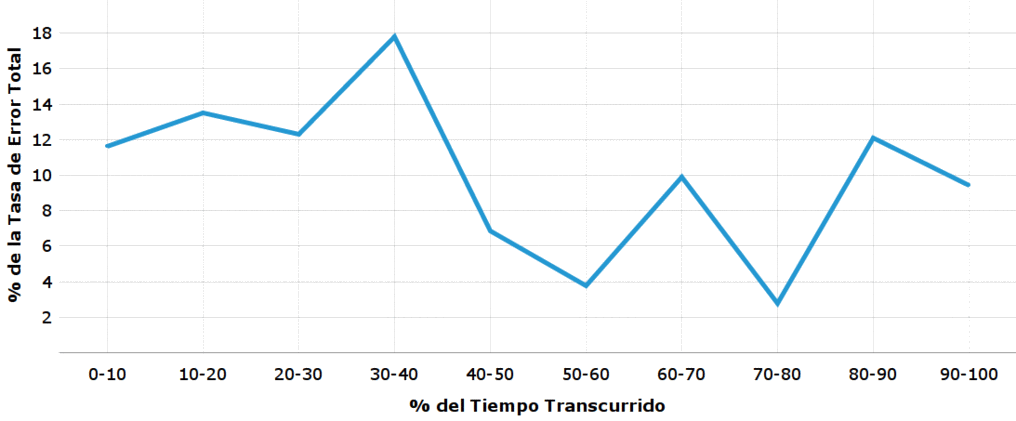
\includegraphics[width=1\linewidth]{./graphics/error_tiempo.png}
\caption{Distribuci\'on del Error Humano por Etapas de la Sesi\'on.}
\label{figure:gerror-tiempo}
\end{figure}
\end{frame}

\begin{frame}{Resultados Obtenidos (6)}
\framesubtitle{An\'alisis del Error Humano}
\begin{table}[H]
\centering
\footnotesize
\caption{Lista de 5 comandos con mayor tasa de error de la aplicaci\'on.}
\begin{tabular}{|l|p{2cm}|}
\hline
Comando & Tasa de Error \\
\hline
crear nueva partitura & 18,38 \\
duplicar pista uno en pista dos & 17,5 \\
duplicar pista uno en pista tres & 16,67 \\
duplicar pista tres en pista cuatro & 13,25 \\
comp\'as cuatro & 13,19 \\
\hline
\end{tabular}
\label{sec:tabla-lista-comandos-error}
\end{table}
\end{frame}


\begin{frame}{Resultados Obtenidos (7)}
\framesubtitle{An\'alisis del Error Humano}
\begin{table}[H]
\centering
\footnotesize
\caption{Tasa de Error Humano por Nivel Contextual del Comando}
\begin{tabular}{|p{2cm}|p{1.6cm}|}
\hline
Nivel Contextual & Tasa de Error \\
\hline
General & 13,25 \\
Pista & 3,57 \\
Comp\'as & 5,16 \\
\hline
\end{tabular}
\label{sec:error-contexto}
\end{table}
\end{frame}


\begin{frame}{Resultados Obtenidos (8)}
\framesubtitle{Encuesta}
Los resultados de la encuesta permiten conocer la apreciaci\'on subjetiva de
los usuarios acerca de su interacci\'on con \foreign{TamTam Listens} y su percepci\'on
sobre las interfaces mediante voz en general.

\begin{table}[H] 
\centering
\footnotesize
\caption{Resumen de la encuesta realizada.}
\begin{tabular}{|l|l|}
\hline
Pregunta & Respuesta Promedio \\
\hline
{?`}Fueron adecuadas las palabras utilizadas? & 6.17 \\
{?`}Fueron adecuados los comandos utilizados? & 6.58 \\
{?`}Fue adecuada la duraci\'on del entrenamiento? & 6.25 \\
{?`}Utilizar{\'\i}as una interfaz por voz en la vida diaria? & 5.83 \\
\hline
\end{tabular}
\label{sec:tabla-encuesta}
\end{table}
\end{frame}
